

\section{The Becker-Gottlieb transfer} % <<<
\label{TheBeckerGottliebTransfer}
\ifx\OutputTheBeckerGottliebTransfer\undefined\else
One of the advantages of a topics course is that you can change direction in midstream.  So now let's study the Adams conjecture for a while, starting with a tool by Becker and Gottlieb which enables us to get a slicker proof than the original ones of Quillen and Friedlander.  It's a construction that's of interest anyway: ``transfer.''  The basic construction is so simple that it's hard to concentrate on it long enough to appreciate how much information it contains.
\begin{enumerate}
\item Pontrjagin-Thom construction: If $X$ is a locally compact Hausdorff space and $U \subseteq X$ is an open subset, then you get a map $\pt{X} \to \pt{X} / (\pt{X} \setminus U) \simeq \pt{U}$ from the one-point compactification of $X$ to that of $U$, just by collapsing out the complement of $U$ in $\pt{X}$.  This is called the ``Pontrjagin-Thom collapse,'' and it gives a contravariance you may not have noticed before.  The construction is natural with respect to proper maps: if $f: X \to X'$ is proper, $U' \subseteq X'$, and $U = f^{-1}(U')$, then you get
\begin{ctikzcd}
\pt{X} \dar\rar["f"] & \pt{X'} \dar\\
\pt{U} \rar["f"] & \pt{U'}
\end{ctikzcd}


\item The Gysin map: Next we apply the Pontrjagin-Thom construction to the case of a smooth fibration of compact manifolds $F \to E \stackrel{p}{\to} B$.  We'd like to convert $p$ to an open embedding.  By the Whitney embedding theorem you can embed $E$ in $\R^n$ for $n$ sufficiently large, and an embedding $E \into \R^n$ induces an inclusion
\begin{ctikzcd}
E \dar["p"']\rar["i"] & B \times \R^n \dlar\\
B
\end{ctikzcd}
Well, $i$ still isn't an open inclusion, so now consider $\nu(i)$ the normal bundle of the inclusion and get a tubular neighborhood $N$ of $E$ in $B \times \R^n$.  Now the Pontrjagin-Thom collapse gives a map
\begin{ctikzcd}
\pt{(B \times \R^n)} \dar[equal]\rar & N_+ \drar[equal]\rar[equal] & T(\nu(i) \downarrow E) \dar[equal]\\
T(n\varepsilon \downarrow B)\dar[equal] & & \Nbar / \partial N \\
\Suspend^n \pt{B}.
\end{ctikzcd}

Lots of Thom spaces are going to appear for a while, so perhaps we should give in and follow Atiyah's convention of writing the bundle as an exponent: $T(\nu(i) \downarrow E) = E^{\nu(i)}$.  So we have a map $B^{n\varepsilon} \to E^{\nu(i)}$.

In some sense what you're going is inverting $p$, constructing a sort of multivalued inverse.  It's instructive to think about the case that $p: E \to B$ is a finite cover.
\begin{figure}[ht!]
\centering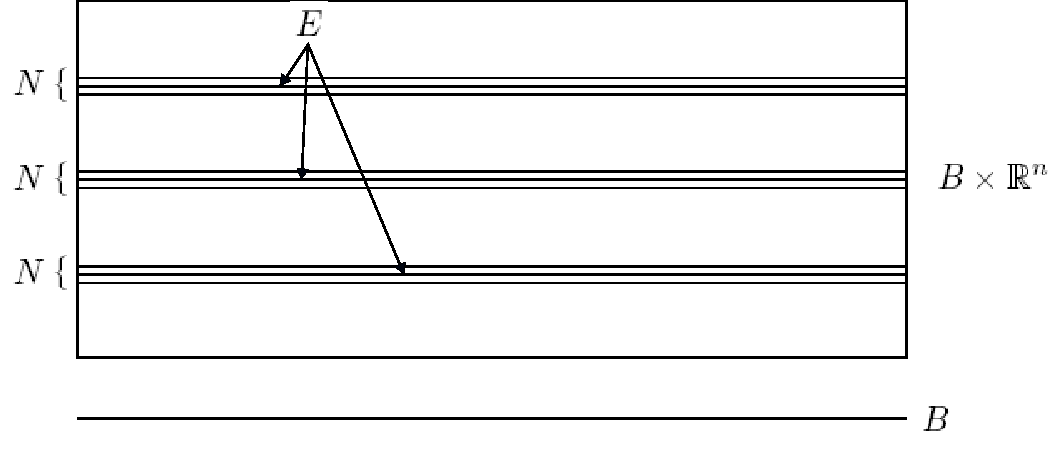
\includegraphics[width=0.4\textwidth]{figures/figure38-1.pdf}
\newline
\centering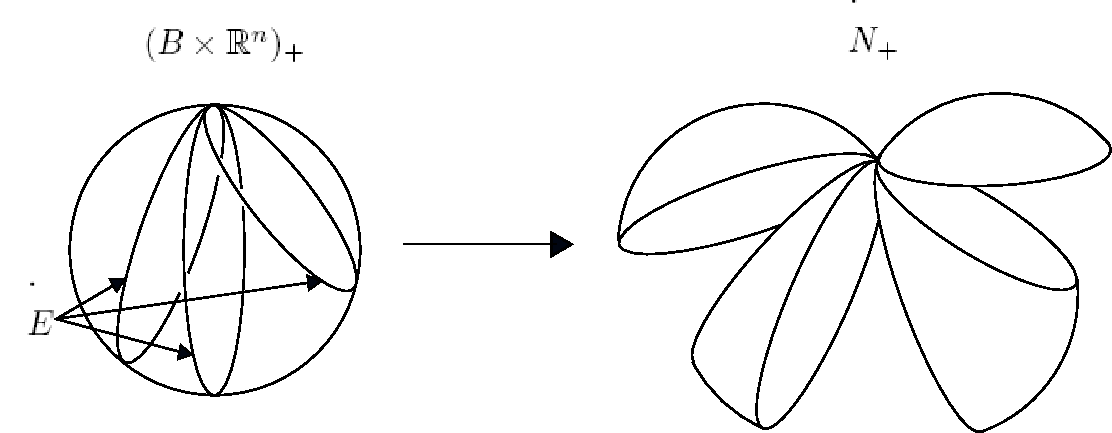
\includegraphics[width=0.4\textwidth]{figures/figure38-2.pdf}
\caption{\small Constructing the Gysin map.}
\end{figure}

The next question is: what is $\nu(i)$?  Well, $\nu(i) + \tau_E = i^*(\tau_{B \times \R^n}) = p^* \tau_B + n\varepsilon_E$.  Now $\tau_E = p^* \tau_B + \tau(p)$, the ``vertical vectors'' or tangent vectors along the fiber.  So $\nu(i) + \tau(p) = n \varepsilon_E$; this is sort of a tangent bundle / normal bundle ``relative to $B$.''  So $\nu(i) = n \varepsilon - \tau(p)$, and so we get a stable map $B_+ \stackrel{p_!}{\stableto} E^{-\tau(p)}$, called the Gysin map, denoted $p_!$ for ``$p$ shriek'' or ``$p$ surprise.''  (We're also going to start writing $\stableto$ from here on out for stable maps.)

\item The Becker-Gottlieb transfer: the inclusion $\nu(i) \into n \varepsilon_E$ induces a map of Thom spaces $E^{\nu(i)} \to E^{n \varepsilon} = \Suspend^n \pt{E}$, which, together with the Gysin map,
\begin{ctikzcd}
\Suspend^n \pt{B} \rar[equal] & B^{n \varepsilon} \rar["p_!"] & E^{\nu(i)} \rar & E^{n \varepsilon} \rar[equal] & \Suspend^n \pt{E}
\end{ctikzcd}
is the Becker-Gottlieb transfer $t(p): \pt{B} \stableto E_+$, which has the virtue that it doesn't shift dimensions.
\item Euler characteristic: The Euler characteristic in this context will be defined as $\chi(p) \in \pi_S^0(B)$, an element in the stable cohomotopy of $B$.  Namely, start with the transfer $t(p): \pt{B} \stableto \pt{E}$.  Now there's a ridiculous map $\pt{E} \to S^0$ which takes the basepoint to the basepoint and pinches everything else (i.e., $E$) to the other point.  On the level of complexes, this isn't much of a map, but the claim is that stably there's a lot going on.  So the Euler characteristic is defined as $\chi(p): \pt{B} \stackrel{t(p)}{\stableto} \pt{E} \stackrel{\mathrm{pinch}}{\to} S^0 \in \pi_S^0(B)$ (i.e., unreduced stable cohomotopy).

Naturality of $\chi(p)$ follows from the naturality of $p_!$ with respect to pullbacks: if $E = f^* E'$ in TERRIBLE DIAGRAM we get $f^* \nu(i') = \nu(i)$, and $N'$ is a tubular neighborhood for $E'$ in $B' \times \R^n$, we can use $f^{-1} N'$ for one of $E$ in $B \times \R^n$ (we may have to choose $N'$ well, but because $B$ and $B'$ and the fiber are compact, there is no real difficulty).  Then we get the following naturality:
\begin{ctikzcd}
B^{n\epsilon} \ar[dd,"t(p)"']\drar["p_!"]\ar[rrr,"f"] & & & (B')^{n\epsilon}\ar[dd,"t(p')"]\dlar["p'_!"']\\
& E^{\nu(i)}\dlar\ar[r,"f"] & (E')^{\nu(i')}\drar\\
E^{n\epsilon} \ar[rrr,"f"] &&& (E')^{n\epsilon}
\end{ctikzcd}
The naturality of $\chi(p)$ follows by pinching out.
\end{enumerate}

We'd like to understand several things; for one, what does the Euler characteristic $\chi(p)$ have to do with the Euler characteristic in the usual sense?  Here's a start:
\begin{lem}
The following diagram commutes:
\begin{ctikzcd}
\pt{B} \dar["\Delta"']\rar[stable,"t(p)"{yshift=0.6ex}] & \pt{E} \rar["\pt{p}"] & \pt{B} \\
\pt{B} \sprod \pt{B} \dar[equal]\ar[rr,"\chi(p) \sprod 1"] & & S^0 \sprod \pt{B}\uar["\cong"'] \\
\pt{(B \times B)}
\end{ctikzcd}
\end{lem}
Before we prove the lemma, note this corollary.  Any cohomology theory has an action of stable cohomotopy: if $\alpha \in \{X, h\}$ is a class in $h^*(X)$ and $\beta \in \pi^S(X) = \{X, S\}$, then we get $\beta \cup \alpha: \Suspend X \to \Suspend X \wsum \Suspend X \stackrel{\Suspend (\alpha \wsum \beta)}{\to} \Suspend (h \wsum S) \to \Suspend h$.
\begin{cor}
If $x \in h^*(B)$, then $t(p)^* (p^* x) = \chi(p) \cup x$.
\end{cor}
\begin{proof}[Proof of the Lemma]
Consider AWFUL DIAGRAM.  Things on the left are the pullbacks of things on the right.  Then we get
\begin{ctikzcd}
B^{n\epsilon} \ar[dd,"t(p)"']\drar\ar[rrrr,"\Delta" xshift=-0.1em] & &[-2em] &[-2em] &[width("$B^{n\epsilon}$")-width("$E^{\nu(i)}\sprod B^0$")+0.6em] B^{n\epsilon}\sprod B^0\dar[dd,"t(p)\sprod 1"]\dlar\\
& E^{\nu(i)}\dlar\ar[rr,"\Delta"] && E^{\nu(i)}\sprod B^0\drar\\
E^{n\epsilon} \ar[drr,"\Suspend^n p"']\ar[rrrr,"\Delta"] &&&& E^{n\epsilon}\sprod B^0 \ar[dll,"\text{collapse $E$}"{sloped,anchor=north}]\\
&& S^N\sprod B^0
\end{ctikzcd}
\end{proof}


Now focus on $\chi(p)$ as a cohomotopy class.  We have
\begin{lem}
In $F \to E \stackrel{p}{\to} B$ the Hurewicz map $\pi^0_S B \to H^0 B$ sends $\chi(p)$ to $\chi(F)$, the usual Euler characteristic of $F$.
\end{lem}
\begin{rem}
Of course it's easier to prove the lemma if you take the right definition of $\chi(F)$.  Notice also that $\chi(p)$ in stable cohomotopy has a lot more information; when you project to cohomology you forget about $p$.
\end{rem}
\begin{proof}
Suppose $B$ is connected; pick a point $\ptspace$ in $B$.  Then $H^0(B) \stackrel{j^*}{\to} H^0 (\ptspace)$ is an isomorphism, and
\begin{ctikzcd}
F\dar["p_F"']\rar & E\dar["p"]\\
\ptspace\rar["j"] & B
\end{ctikzcd}
is a pullback, so $j^* \chi(p) = \chi(p_F)$.  So we can assume $B = \ptspace$.  The only space left is $F$.  Given an embedding $i: F \into S^n$, the Euler characteristic $\chi(p)$ is defined by $S^n \stackrel{p_!}{\to} F^{\nu(i)} \to F^{\nu(i) \oplus t(F)} \stackrel{\mathrm{pinch}}{\to} S^n$, and we must show this composite has degree $\chi(F)$.

Let $N \subset \R^n$ be a tubular neighborhood for the embedded image of $F$; then $S(\nu) = \partial N$, and $\partial N$ is a codimension - 1 submanifold with an outward-pointing normal direction.  The map $F^\nu \to S^n$ is the Thom-space level of a map
\begin{ctikzcd}
\nu\dar\rar & \nu\oplus\tau \dar\rar & \R^n\dar\\
F \rar & F \rar & \ptspace
\end{ctikzcd}
which on the level of sphere-bundles is a map $\gamma: \partial N \to S^{n-1}$, the Gauss map!  The degree of $\gamma$ is a standard definition of the Euler characteristic $\chi(F)$; see Milnor~\cite{Milnor} for further information.  But that's it:
\begin{ctikzcd}
S(\nu)\dar\rar["\gamma"]  & S^{n-1}\dar\\
D(\nu)\dar \rar["\gamma"] & D^n\dar\\
F^\nu \rar & S^n
\end{ctikzcd}
and the bottom pieces receive a map $S^n \to F^\nu$, the Pontrjagin-Thom collapse (which is degree 1 by construction), and the composite $S^n \to S^n$ has degree $\chi(F)$.
\end{proof}

It's worth thinking about this on the level of cohomology.  The bundle maps
\begin{ctikzcd}
\nu \dar["\zeta"']\rar{\Delta} & \{0\}\times\nu\dar{\zeta\times 1}\\
n \rar{\Delta} & \tau\times\nu
\end{ctikzcd}
induce on the level of Thom spaces
\begin{ctikzcd}
F^{\nu} \dar["\zeta"']\rar & F^0 \sprod F^\nu\dar{\zeta\times 1}\\
F^{n\varepsilon} \rar & F^{\tau}\sprod F^{\nu}
\end{ctikzcd}
If $u \in \Htwee^n(X^\xi)$ is the Thom class of $\xi$ define the Euler class $e_\xi$ as the image under pullback by $\zeta$:
\begin{ctikzcd}[row sep=0em]
\Htwee^n X^\xi \rar{\zeta^*} & \Htwee^n(X^0) \rar[equal] & \Htwee^n(X) \\
u_\xi  \rar[mapsto] & e_\xi.
\end{ctikzcd}
Then in the above square, the Thom classes go
\begin{ctikzcd}
e_\tau \cup U_\nu & \lar[mapsto] e_\tau \sprod U_\nu \\
U_{n \varepsilon} \uar[mapsto,"\zeta"]& \lar[mapsto] U_\tau \sprod U_\nu \uar[mapsto]
\end{ctikzcd}
Let $\sigma \in \Htwee^n S^n$ be a generator; think of it as the Thom class of $\R^n$ over $\ptspace$.  The diagram
\begin{ctikzcd}
\nu\dar\rar & \nu\oplus\tau \dar\rar & \R^n\dar\\
F \rar & F \rar{\text{pinch}} & \ptspace
\end{ctikzcd}
gives maps of Thom spaces under which $\sigma$ pulls back as
\begin{ctikzcd}[row sep=0em]
S^n\rar{c} & F^{\nu}\rar & F^{\nu\varepsilon} \rar & S^n\\
\chi(F)\cdot\sigma &\lar[mapsto] e_\tau \cup U_\nu & \lar[mapsto] U_{n\varepsilon} & \lar[mapsto] \sigma
\end{ctikzcd}
We can use classical theorems about the Euler characteristic to study our new Euler characteristic; for example, we can use Hopf's theorem to compute it in a special case.

\begin{wrapfigure}{r}{0.25\textwidth}
\centering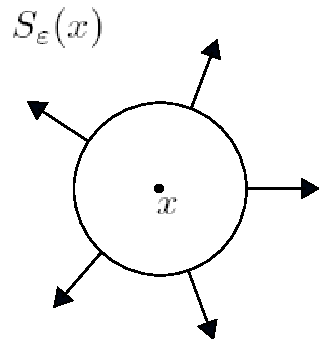
\includegraphics[width=0.25\textwidth]{figures/figure39.pdf}
\caption{\small Picture of $S_\epsilon$ about a zero at $x$.}
\end{wrapfigure}
Let $M^n$ be a compact Riemannian manifold and let $v$ be a non-degenerate vector field (i.e., $v(M)$ intersects the zero section $\zeta(M)$ of $TM$ transversally).  Then around each zero $x$ of $v$ there is a small sphere $S_\epsilon(x)$ so that $V|_{S_\epsilon(x)} \ne 0$.  Define $i_x$ to be the degree of $\frac{v}{\|v\|}|_{S_\epsilon(x)}: S^{n-1}_\epsilon \to S^{n-1} = \pm 1$.
\begin{thm}[Hopf]
$\chi(M) = \sum_{\substack{x \in M \\ v(x) = 0}} i_x$.
\end{thm}
\begin{proof}
(See Milnor~\cite{Milnor}.)
\end{proof}
For example, suppose $G$ is a compact Lie group; let $T \subset G$ be a maximal torus; let $N(T)$ be its normalizer.  Then the identity component of $N(T)$ is $T$ itself, and $N(T) / T$ is a finite discrete group, the ``Weyl group.''  The important claim is that $\chi(G / T) = |W|$ and $\chi(G / N(T)) = 1$ if $G$ is compact and connected.

To prove this, we'll come up with a vector field and use Hopf's theorem.  There is an action of $G$ on $G/T$ which restricts to an action of $T$.  In $T_eT = L(T)$ the Lie algebra of $T$ there is a vector $x$ such that $\exp x = g$, and $\exp tx$ is a path in $T$ from $e$ to $g$; let $\gamma_t$ be the induced flow on $G/T$; then $\frac{d}{dt} \gamma_t |_{t = 0}$ is a vector field on $G/T$.  Now suppose $g \in T$ is such that $\{g^n \mid n \in \Z\}$ is dense in $T$ (i.e., $g$ is irrational on each component of the torus; $T$ is called ``topologically cyclic''); let $v$ be the vector field on $G/T$ corresponding to this element.  A zero of $v$ is a fixed point of the action of $g$ and therefore (by continuity) a fixed point for the action of $T$.  Such a point in $G/T$ is a coset $hT$ so that $thT = hT$ for all $t \in T$, equivalently $hth^{-1} T = T$ for all $t \in T$, equivalently $h$ lies in the normalizer of $T$.  So zeroes correspond to elements of $N(T) / T = W$.  I claim all the zeroes are non-degenerate and have the same index, so $\chi(G/T) = |W|$.  Now the action of $g$ descends to $G/N(T)$ with only one fixed point, so $\chi(G/N(T)) = 1$.

Now let's talk about the transfer in $\K$-theory.  Suppose $p: E \to B$ is a finite covering.  Then the transfer is a map $t(p): B^{n \varepsilon} \to E^{n \varepsilon}$ which induces a map in $\KO$-theory $\KO(E) \to \KO(B)$.  There's an obvious thing to do here, but there's no obvious connection with the map $t(p)$: if $\xi$ over $E$ is a vector bundle, we can form a vector bundle over $B$ by taking as fiber over $b \in B$ the sum of the vector spaces over points in $E$ which cover $b$:
\begin{ctikzcd}[display math]
b \in B \rar[wavy]& \bigoplus_{p(x) = b} \xi_x = (p_* \xi)_b
\end{ctikzcd}

This is more than you might hope for; it says there's an underlying map $\mathrm{Vect}(E) \to \mathrm{Vect}(B)$.  But in fact, the two constructions are the same:
\begin{lem}[Nontrivial]\todo{Either should prove it or at least explain what's hard in the proof.}
\begin{ctikzcd}
\KO(E) \rar["t(p)^*"] & \KO(B) \\
\Vect(E) \uar[hook]\rar["p_*"] & \Vect(B)\uar[hook].
\end{ctikzcd}
\end{lem}
\begin{cor}
Let $p: E \to B$ be a finite covering and $\xi \in \KO(B)$; then if $\xi$ is stably fiber-homotopy trivial, so is $t(p)^* \xi$.
\end{cor}
\begin{rem}
Note that this isn't a trivial fact: transfer is a cohomological construction but stable fiber homotopy triviality isn't.  But it follows from the lemma: a map $S(\xi) \to S^{n-1}$ which is degree 1 on each fiber gives a map $S(p_* \xi) \to S^{n - \deg p}$ which is degree one on each fiber.
\end{rem}
\begin{rem}
The corollary can also be proved by noticing the factorization
\begin{ctikzcd}
\KOtwee(X) \dar[onto]\rar & \Sphtwee(X) \\
\Jtwee(X)\urar[into]
\end{ctikzcd}
and that $\Sphtwee = \Sphtwee^0$ is the zeroth level of a cohomology theory, using the infinite loop space theory of Boardman and Vogt.  So the transfer maps induce maps in this theory, and you can produce the result by a naturality argument.
\end{rem}

The second fact about transfer in $\K$-theory is the relation to Adams operations.  In fact, the result really concerns the interaction of Adams operations with arbitrary stable maps.
\begin{lem}
Suppose $f: \pt{x} \stableto \pt{Y}$ ; then $f^* \psi^k x - \psi^k f^* x$ has order dividing a power of $k$ (and independent of $x$).  In particular, the Adams operations are unstable.
\end{lem}
\begin{proof}
To study the problem, you have to distinguish between the stable map $f$ and an actual representative.  Let $f^*: \KO(\pt{Y}) \to \KO(\pt{X})$ denote the induced homomorphism.  Pick $n$ large enough so that there is an actual map $f: \pt{X} \sprod S^{8n} \to \pt{Y} \sprod S^{8n}$.  Then
\begin{cjointikzcd}
\diagram x\dar[mapsto]\\x\otimes\gamma^n
%
\diagram
    \KOtwee(\pt{X}) \dar{\cong}& \lar["f^*"'] \KOtwee(\pt{Y})\dar{\gamma^{\otimes n}} \\
    \KOtwee(\pt{X}\sprod S^{8n}) &  \lar["f^*"'] \KOtwee(\pt{Y}\sprod S^{8n})
\end{cjointikzcd}\todo[noline]{Check that this diagram is right.}
with $\gamma$ a generator of $\KOtwee(S^8) \cong \Z$.  Choosing this, you find
\begin{align*}
\psi^k(f^*(x) \otimes \gamma^n) & = \psi^k(f^*(x \otimes \gamma^n)) \\
k^{4n} \psi^k f^*(x) \otimes \gamma^n & = f^* \psi^k(x \otimes \gamma^n) \\
& = f^*(\psi^k x \otimes k^{4n} \gamma^n) \\
& = k^{4n} f^*(\psi^k x \otimes \gamma^n) \\
& = k^{4n} (f^* \psi^k x) \otimes \gamma^n.
\end{align*}
So $k^{4n}(\psi^k f^* - f^* \psi^k) = 0$, and $n$ depended only on $f$.
\end{proof}

% >>>
\fi
\BoxedNote{}

\section{The Adams conjecture} % <<<
\label{TheAdamsConjecture}
\ifx\OutputTheAdamsConjecture\undefined\else
To make greatest use of most constructions in algebraic topology, it is generally helpful to have a relative version.  This time, we'll use a relative version of the transfer map.  So, as before, let $F \to E \stackrel{p}{\to} B$ be a smooth fiber bundle with $F$ and $B$ compact; let $\xi$ over $B$ be a vector bundle, and consider
\begin{ctikzcd}
p^* \xi \dar\rar & \xi\dar \\
E \rar["p"] & B.
\end{ctikzcd}
As before, we pick an embedding $E \into \R^n$ and get
\begin{ctikzcd}
E \dar["p"']\rar[into] & B \times \R^n \dlar["\pr"]\rar[into]{\zeta} & n \varepsilon \oplus \xi \\
B.
\end{ctikzcd}
Now embed one step farther: $\zeta: B \times \R^n \into n \varepsilon \oplus \xi$.  And we can do the collapse on the inclusion given by a tubular neighborhood for $p^* \xi$ in $n \varepsilon \oplus \xi$:
\begin{ctikzcd}
\Suspend^n B^\xi \ar[rrr,bend right=10,yshift=-0.2em, "t(p)"']\rar["p_!"] &  E^{\nu(i) \oplus p^* \xi} \rar[into] & E^{n \varepsilon \oplus p^* \xi} \rar[equal]& \Suspend^n E^{p^* \xi}
\end{ctikzcd}
The relative transfer is the corresponding stable map $t(p): B^\xi \stableto E^{p^* \xi}$.
\begin{lem}
Suppose $\chi(F) = \pm 1$.  In that case, if $\J(p^* \xi) = 0$ in $\J(E)$, then $\J(\xi) = 0$ in $\J(B)$, so $p$ is a monomorphism on $J$-theory.
\end{lem}
\begin{proof}
$\J(p^* \xi) = 0$ means that
\begin{ctikzcd}
S^d \rar & E^{p^* \xi} \rar[stable,"\exists"{yshift=0.6ex}] & S^d
\end{ctikzcd}
where the composite has degree 1 and $d$ is the dimension of $\xi$.  Then we have
\begin{ctikzcd}
S^d \rar & E^{p^* \xi} \rar[stable] & S^d \\
& B^{\xi}\uar["t(p)"'] & \lar S^d
\end{ctikzcd}
and we'd like to show the degree of this right-hand composite is $\pm 1$.  Well, choose a basepoint in $B$; then you have
\begin{ctikzcd}
d\varepsilon \ar[dd]\ar[dr]\ar[rr] & & p^*\xi\ar[dd]\ar[dr]\\
& F\ar[rr]\ar[dd] && E\ar[dd]\\
\R^d \ar[rr]\ar[dr] && \xi\ar[dr]\\
& \ptspace \ar[rr,into] && B
\end{ctikzcd}
and from this you get
\begin{ctikzcd}
F^{d\varepsilon} \rar & E^{p^* \xi}  \rar[stable]& S^d \\
S^d \uar[stable] \rar & B^\xi\uar[stable].
\end{ctikzcd}
But $S^d \stableto F^{d \varepsilon}$ isn't just the inclusion of the bottom cell; in fact, we found that it was $\chi(F)$ times the inclusion of the bottom cell!  So if $\chi(F) = \pm 1$, $S^d \to B^\xi \stackrel{t(p)}{\to} E^{p^* \xi} \stableto S^d$ has degree one.

But \begin{tikzcd}S^d \rar[stable]& F^{d \varepsilon}\end{tikzcd} isn't just the inclusion of the bottom cell; in fact, we found that it was $\chi(F)$ times the inclusion of the bottom cell!  So if $\chi(F) = \pm 1$, the composition
\begin{ctikzcd}S^d \rar & B^\xi \rar["t(p)"] & E^{p^* \xi} \rar[stable]& S^d\end{ctikzcd}
has degree one.
\end{proof}

Now I'm ready to tell you what the Adams Conjecture says, although not what it means: let $B$ be a finite complex, let $\xi \in \KO(B)$, and let $k \ge 1$ an integer.  Then some power of $k$ kills $\J(\psi^k \xi - \xi)$ in $\J(B)$.

Admittedly, this is an obscure statement, but take it from me that it's important and worth proving.  We'll prove it bit by bit.
\begin{enumerate}
\item $\xi$ is a linear combination of line bundles.  If $k$ is odd then $\psi^k \xi = \xi$ so $\psi^k \xi - \xi = 0$.  If $k$ is even and $\xi$ is a line bundle (by additivity it's sufficient to consider this case), then $\psi^k \xi - \xi = 1 - \xi \in \KOtwee(B)$.  $\xi$ is classified by a map $f: B \to \RP^N$ for large enough $N$:
\begin{ctikzcd}
\xi \dar\rar & L\dar \\
B \rar["f"] & \RP^N,
\end{ctikzcd}
so $1 - \xi = f^*(1 - L)$, and $\KOtwee(\RP^N)$ is a finite 2-group generated by $(1-L)$.
\item The next case is that $\xi$ is a $2$-dimensional bundle.  Let $P$ be the associated principal bundle so that $\xi  = P \times_{O(2)} \R^2$.  We described the Adams operations $\psi^k$ in terms of representations, so now we have to think a little about the representation theory of $O(2)$: what is $O(2)$?  Well, there are two parts:
\begin{ctikzcd}
S^1 \rar & SO(2) \rar[into] & O(2) \rar[yshift=0.2em] & \lar[yshift=-0.2em] \Z_2,
\end{ctikzcd}
where the splitting comes from choosing any reflection, say $r$ is the reflection through the $x$-axis.

So what are the representations of $O(2)$?  Let $V = \R^2$ be the basic representation; then we can take exterior powers:
\begin{align*}
\lambda^0(V) & = 1, \\
\lambda^1(V) & = V, \\
\lambda^2(V) & = \det.
\end{align*}
More interestingly, we have representations $\mu_k$ given by $S^1$ acting on $\C^{\otimes_\C k}$ by, for $z \in S^1$, $z \cdot (w_1 \otimes \cdots \otimes w_k) = zw_1 \otimes \cdots \otimes zw_k = z^k(w_1 \otimes \cdots \otimes w_k)$, and we can extend to $O(2)$ by letting $r$ act by complex conjugation.  Note that $\mu_1 = V$.

Next we want to express the $\psi^k$s in terms of $\lambda^j$s and $\mu_k$s, so that we have some chance of being able to compute.  In order to do that, we should write down the character table for $O(2)$:
WHAT A MESS\todo{It seems like in a lot of these all caps places, we're missing things...} $\mu_k$ is the natural candidate for $\psi^k$, but it's wrong: the formula for $\psi^k$ is
\[
\psi^k = \begin{cases} \mu_k & \hbox{if $k$ is odd,} \\ \mu_k + (\lambda_0 - \lambda_2) & \hbox{if $k$ is even.} \end{cases}
\]

Now we can use the $\mu_k$s to check the Adams conjecture: $\psi^k V - V$ differs from $\mu_k V - V$ by a linear combination of line bundles with virtual dimensions $0$ (assuming $k$ is even); these are killed by a power of 2 by the above argument for the line bundle case.  if $k$ is odd, $\psi^k V - V = \mu_k V - V$.  The claim is that for some $e$, $k^e(\mu_k V - V) = 0$ in $J$.

The trick --- which is the key point in understanding the Adams conjecture --- is the map $f_k: V \to \mu_k$ given by $f_k(z) = z^k$, which is equivariant with respect to the $O(2)$ action on either side, but certainly not linear; it won't induce a map of vector bundles, but it will induce one of sphere bundles, which is degree $k$ on each fiber.  The result then follows from
\end{enumerate}
\begin{lem}[Adams' Mod $k$ Dold Lemma, Adams, $\J(X)$ I, Topology around 1965]
Let $B$ be a finite complex and let $\xi, \xi'$ be vector bundles over $B$.  Suppose $f: S(\xi) \to S(\xi')$ is degree $k$ on each fiber.  Then $k^e(\J(\xi) - \J(\xi')) = 0$ for some $e$.
\end{lem}

This is as far as Adams got; he decided it was unreasonable of others to expect him to do more.  Now you need a trick to be able to finish in a finite amount of time.

To do the general case we'll make a few reductions, namely to oriented $2n$-dimensional bundles.  A vector bundle $\xi$ over $B$ has a Stiefel-Whitney class $w_1(\xi) \in H^1(B; \Z_2)$ which is the obstruction to the orientability of $\xi$.  Now elements of $H^1(B; \Z_2)$ are in one-to-one correspondence via $w_1$ with line bundles.

Now perform the $L$ and $\Ltwee$ constructions fiberwise on the bundle $\xi$ over $B$ and you get a fiber bundle
\begin{ctikzcd}
               & \Ltwee(\xi) \dar["q"']&\lar \zeta\\
L(\R^{2n})\rar & L(\xi)\dar["p"'] & \lar p^*\xi\\
               & B                &\lar\xi
\end{ctikzcd}
where $L(\R^{2n})$ has $\chi = 1$ and $\zeta$ is two plane bundles.  The claim is that this wonderful formula is geometrically clear: $t(q)^* \zeta = q_* \zeta = p^* \xi$ over $B$, so in particular there is a line bundle $\lambda$ over $B$ so that $w_1(\xi \oplus \lambda) = 0$, i.e., $\xi \oplus \lambda$ is orientable.  The additivity of the Adams conjecture (plus the fact that we've already proved it for line bundles) implies that we can assume $\xi$ is an oriented, $2n$-dimensional vector bundle over $B$; moreover $B$ is compact so we can give $\xi$ a metric.

Now suppose $B$ is a $2n$-dimensional inner product space over $\R$; let $F(V)$ be the space of sequence of $n$ mutually orthogonal $2$-planes in $V$.  $\Sigma_n$ acts freely on $F(V)$; let $L(V) = F(V) / \Sigma_n$.  I claim we've constructed this space before as $SO(2n)/NT$.  So $\chi(L(V)) = 1$.

Now let $\Sigma_{n-1}$ act on $F(V)$ by fixing the last element; then there is an $n$-sheeted cover $\Ltwee(V) = F(V)/\Sigma_{n-1} \stackrel{q}{\to} L(V)$.  Moreover, there is a $2$-plane bundle $\zeta$ over $\Ltwee(V)$ defined fiberwise by setting $\zeta_{(\{v_1, \ldots, v_{n-1}\}, v_n)} = v_n$.  Now from the lemma at the beginning of this lecture, it suffices to check the Adams conjecture on $p^* \xi$.  But by the formula,
\begin{align*}
\psi^k p^* \xi - p^* \xi & = \psi^k t(q)^* \zeta - t(q)^* \zeta \\
& = \psi^k t(q)^* \zeta - t(q^* \psi^k \zeta + t(q)^* \psi^k \zeta - t(q)^* \zeta \\
& = (\psi^k t(q)^* - t(q)^* \psi^k) \zeta + t(q)^*(\psi^k \zeta - \zeta).
\end{align*}
The left summand is killed by $k^e$ and the right summand is killed by $k^f$ for some $f$ by the proof of the adams conjecture for $2$-plane bundles.

% >>>
\fi
\BoxedNote{}

\section{Some summands of the stable homotopy groups of spheres} % <<<
\label{SomeSummandsOfStableHomotopyOfSpheres}
\ifx\OutputSomeSummandsOfStableHomotopyOfSpheres\undefined\else
All right, today we'll study the meaning of the Adams conjecture; in particular I'm going to tell you about the space $J$.  We've talked about the $\KO$ spectrum, representing real $\K$-theory: $\KO^*(X) = \{X, \KO\}$.  It is a sequence of spaces $\{\KO_n\}$ with maps $\alpha_n: \Suspend \KO_n \to \KO_{n+1}$, with
\begin{align*}
\KO_{8n} & = \Z \times BO \\
\KO_{8n-i} & = \Loops^i (\Z \times BO) \\
\Suspend^8 \KO_{8n} & \to \KO_{8n+8} \hbox{ is given by}
\end{align*}
\begin{ctikzcd}
S^8 \sprod (\Z \times BO) \dar\rar & \Z \times BO \\
(\Z \times BO) \sprod (\Z \times BO)\urar["\mu"].
\end{ctikzcd}
Bott periodicity says $\Z \times BO \stackrel{\simeq}{\to} \Loops^8(\Z \times BO)$.

Now $\KO(X)$ is a ring with unit; $\KOtwee^0(S^0) \cong \Z \ni 1$.  So there is a map of spectra $\Suspend^\infty S^0 = S \to \KO$ representing $1 \in \KOtwee(S^0)$.  One question is, how big is the image of the induced map $\pi_*^S \to \KO_*$?

Another way to ask this question is this: every spectrum has a space associated with it; in this case, we get a map $QS^0 = \Loops^\infty \Suspend^\infty S^0 \to \Z \times BO$ whose effect in unstable homotopy is the stable homotopy of the map above.  Viewed in this light, the answer depends on self-maps of $\Z \times BO$.  We have the $\psi^k$s, so we should use them.  The operation $\psi^k: \KO \to \KO$ corresponds to a map $\psi^k: \Z \times BO \to \Z \times BO$.  We know the effect of $\psi^k$ on $\pi_*$:
\[
\begin{array}{c|cc}
* & \pi_*(\Z \times BO) & \psi^k \\
\hline
0 & \Z \\
1 & \Z_2 \langle \eta \rangle & \eta \mapsto k \eta \\
2 & \Z_2 \langle \eta^2 \rangle & \eta \mapsto k^2 \eta \\
3 & 0 \\
4 & \Z \langle g_4 \rangle & g_4 \mapsto k^{2k} g_4 \\
5 & 0 \\
6 & 0 \\
7 & 0 \\
8 & \Z \langle g_8 \rangle & g_8 \mapsto k^4 g_8.
\end{array}
\]
Everything else on the table follows from periodicity.

These operations suffer from a bad defect: they're not stable.  But we've already seen how to study this problem when we were studying transfer: namely,
\begin{ctikzcd}[column sep=large]
S^8 \sprod (\Z \times BO) \dar["g_8\sprod 1"']\rar["k^4 \sprod \psi^k"] & S^8 \sprod (\Z \times BO)\dar \\
(\Z \times BO) \sprod (\Z \times BO) \dar["\mu"']\rar["\psi^k \sprod \psi^k"] & (\Z \times BO) \sprod (\Z \times BO)\dar \\
\Z\times BO\rar["\psi^k"] & \Z\times BO
\end{ctikzcd}
By adjunction, we get
\begin{ctikzcd}
\KO_0 \dar["\simeq"']\rar["k^4 \psi^k"] & \KO_0\dar["\simeq"] \\
\Loops^8 \KO_8 \rar["\psi^k"] & \Loops^8 \KO_8.
\end{ctikzcd}
The diagram measures how far $\psi^k$ is from being stable.  The fix we shall use here is to localize so that $k$ becomes a unit.

The point is, $\KO^*$ is a nice ring, so localization is easy to do: $R \subseteq \Q$ is flat over $\Z$, so we can take $\KO^*(X; R)$ to be defined as $\KO^*(X) \otimes_{\Z} R$; e.g., $R = \Z[\frac{1}{k}]$.  Then the diagram becomes
\begin{ctikzcd}[column sep=large]
\KO_0 \dar\rar{\psi^k} & \KO_0 \dar\\
\Loops^8 \KO_8 \rar["k^{-4} \Loops^8 \psi^k"{yshift=0.1em}] & \Loops^8 \KO_8 \left[ \frac{1}{k} \right],
\end{ctikzcd}
i.e., we can define a new operation $\Psi^k: \KO \to \KO[\frac{1}{k}]$ so that
\[
\Psi^k_{8n} = k^{-4n}\psi^k : \Z \times BO \to \Z \times BO \left[ \frac{1}{k} \right]
.\]
Now $\Z[\frac{1}{k}] \into \Z_{(2)}$, assuming $2 \nmid k$, so you get
\begin{ctikzcd}
\KO^* \dar\rar{\Psi^k} & \KO^* \left[ \frac{1}{k} \right]\dar \\
\KO^*_{(2)} \rar{\Psi^k} & \KO^*_{(2)},
\end{ctikzcd}
for $k$ odd.  Take the case $k = 3$ for the rest of this lecture.  But we're still not done massaging the Adams operations; we need the notion of a ``connective cover:'' if $X$ is a space, then its $n^\textup{th}$ connective cover is the space $X \langle n, \ldots, \infty \rangle \to X$, where this map is an isomorphism on $\pi_i$ for $i \ge n$ and $\pi_i X \langle n, \ldots, \infty \rangle = 0$ for $i < n$.  For example, you have
\begin{ctikzcd}
\cdots \rar & BSpin \rar & BSO \rar & BO \rar & \Z \times BO
\end{ctikzcd}
as a sequence of connective covers.  You can do this for spectra, in which case it's interesting to take away negative homotopy groups: $E \langle 0, \infty \rangle_n = E_n \langle n, \infty \rangle$ has no negative homotopy groups.  For example, $\KO$ has negative homotopy groups; its $0$-connective cover localized at $2$ is $\KO \langle 0,\infty \rangle_{(2)} = bo$, called ``connective real $\K$-theory.''  So
\[
\begin{array}{c|ccccccccc}
* & 0 & 1 & 2 & 3 & 4 & 5 & 6 & 7 & (8) \\
\hline
\pi_* bo & \Z_{(2)} & \Z_2 & \Z_2 & 0 & \Z_{(2)} & 0 & 0 & 0
\end{array}
\]
but now we restrict to $* > 0$.  The construction of $\Psi^k$ gives an operation on connective real $\K$-theory $\Psi^k: bo \to bo$ and we know its effect on homotopy groups ($k = 3$ in what's to follow):
\begin{ctikzcd}[column sep=0.6em]
0 & 1 & 2 & 3 & 4 & 5 & 6 & 7 & 8 & 9 & 10 & 11 & 12 & 13 & 14 & 15 & 16 \\[-1.8em]
\Z_{(2)}\dar["\cong"] & \Z_2\dar["\cong"] & \Z_2\dar["\cong"] & 0 & \Z_{(2)}\dar{\cdot9} & 0 & 0 & 0 & \Z_{(2)}\dar{\cdot81} & \Z_2 & \Z_2 & 0 & \Z_{(2)} \dar{\cdot729}& 0 & 0 & 0 & \Z_{(2)} \dar{\cdot9^4}\\
\Z_{(2)} & \Z_2 & \Z_2 & & \Z_2 & & & & \Z_{(2)} & \Z_2 & \Z_2 & & \Z_{(2)} & & & & \Z_{(2)}.
\end{ctikzcd}
Notice that $\Psi^3$ induces the identity in dimensions below $4$.  So consider the map $\Psi^3 - 1: bo \to bo$; now the map acts as $0, 0, 0, \ldots, \cdot 9 - 1, \ldots, \cdot 81 -1, \ldots$ in homotopy.  You could just take the fiber of this map, but because $\Psi^3 - 1$ induces zero in homotopy in dimensions one and two you would get copies of $\Z_2$ from both ends, and these are in fact unnecessary: the map $\Psi^3 - 1$ lifts to the $4$-connective cover\footnote{Why? I need to check the obstruction theory here.}
\begin{ctikzcd}
& bo \langle 4, \infty \rangle\dar \\
bo \urar[dashed]{\exists \varphi} \rar["\Psi^3 - 1"'] & bo
\end{ctikzcd}
and that brings us to the space $J$ --- or at least the spectral $j$.  Set $j$ to be the fiber of $\varphi: bo \to bo \langle 4, \infty \rangle$.  The space $J$ comes from the $0$-space:
\begin{ctikzcd}
\Z \times J \rar & \Z \times BO \rar["\varphi"] & BSpin \\
J \rar & BO\uar[into]\rar & BSpin.
\end{ctikzcd}

OK, we can figure out the homotopy of $J$ because we know about all the things that go into it.  Recall that $\nu(9^k - 1) = \nu(k) + 3$, so $9^k - 1$ is an odd multiple of $2^{\nu(k) + 3}$, or equivalently an odd multiple of $8k$.  Hence $\Psi^3 - 1$ acts either as $0$ or as multiplication by $8k$ and by a unit in $\Z_{(2)}$.  So we get
\begin{ctikzcd}
& 0 & 1 & 2 & 3 & 4 & 5 & 6 & 7 \\
\pi_* J & \Z_{(2)}\dar & \Z_2\dar & \Z_2\dar & \Z_8\dar & 0\dar & 0 & 0 & \Z_{16} \\
\pi_* bo & \Z_{(2)}\dar["0"] & \Z_2\dar["0"] & \Z_2\dar["0"] & 0 & \Z_{(2)}\dar["\cdot9-1"] & 0 & 0 & 0 \\
\pi_* bo \langle 4, \infty \rangle & 0 & 0 & 0 & 0 & \Z_{(2)} & 0 & 0 & 0\\[3em]
%
& 8 & 9 & 10 & 11 & 12 & 13 & 14 & 15 & 16 \\
\pi_* J & \Z_2\dar["0"] & \Z_2^2\dar & \Z_2 & \Z_8 & 0 & 0 & 0 & \Z_{32} & \Z_2 \\
\pi_* bo & \Z_{(2)}\dar["\cdot 81-1"] & \Z_2\dar["0"] & \Z_2\dar["0"] & 0 & \Z_{(2)}\dar["\cdot 9^3-1"] & 0 & 0 & 0 & \Z\dar["\cdot 9^4-1"] \\
\pi_* bo \langle 4, \infty \rangle & \Z_{(2)} & \Z_2 & \Z_2 & 0 & \Z_{(2)} & 0 & 0 & 0 & \Z.
\end{ctikzcd}

What's the point?  The point is, this has to do with homotopy groups of spheres.  You have
\begin{ctikzcd}
 & S^0\dlar\dar \\
j \rar & bo \rar["\varphi"] & bo \langle 4, \infty \rangle
\end{ctikzcd}
and the question is, how big is the image $\pi_* S^0 \to \pi_* J$?  The Adams conjecture answers this.

How?  The adams conjecture says that for some $e$, $3^e \K(\Psi^3 - 1) = 0$.  There is an inclusions $O(n) \into G_n$ ( = all degree $\pm 1$ self-maps of $S^{n-1}$) which is compatible with the inclusions $O(n) \into O(n+1)$ and $G_n \into G_{n+1}$.  So you get a map of the limits $J: O \to G = Q_{\pm} S^0$ which is an $H$-map.  So you get a map of classifying spaces $BJ: BO \to BG$.  Then the Adams conjecture implies that the composite
\begin{ctikzcd}[sep=large]
BSpin \rar & BO \rar["BJ"] & BG_{(2)} \\
 & \ular["\varphi"]BO\uar["\Psi^3-1"'] \urar["\sim *"'].
\end{ctikzcd}
This gives you a map $\alpha$ below:
\begin{ctikzcd}
J \dar["\alpha"']\rar & BO \dar\rar["\varphi"] & BSpin\dar \\
G \rar & EG \rar & BG_{(2)}.
\end{ctikzcd}
Now in fact $\alpha$ factors through the $+1$ component of $G$, $SG = Q_1 S^0$:
\begin{ctikzcd}[row sep=0pt]
    & J \dlar["\alpha"]\ar[dd,"\alpha"]\rar & BO \ar[dd]\rar & BSpin \ar[dd]\\
SG \drar\\
   & G \rar & EG \rar & BG_{(2)}.
\end{ctikzcd}
Well, this looks good, in fact it looks very good: the map $S^0 \to j$ is, after you apply $\Loops^\infty$ to it, a map $u: QS^0 \to \Loops^\infty j = \Z \times J$.  And in fact
\begin{ctikzcd}
J \ar[drr,"!!\simeq!!"']\rar["\alpha"] & SG \rar[into] & QS^0\dar["u"] \\
&& J
\end{ctikzcd}
So if $C$ is the fiber of $u$, then there is a homotopy equivalence $QS^0 = SG \simeq J \times C$.  Thus all of the homotopy of $J$ listed above appears as a direct summand in $\pi_* SG$, and in particular in the iamge of $S^0 \to j$.

One game you can play now is to try to get out some information on unstable homotopy.  First we'll need some names: pulling back the sequence $J \to BO \to BSpin$ once, you get $Spin \stackrel{J}{\to} J \to BO$ (where $J$ is essentially the $J$-homomorphism, in the sense that it restricts from $\alpha$).  It's time for another table:
\[
\begin{array}{cccccc}
& \pi_* Spin & \pi_* J & \pi_* BO & \hbox{New names} & \hbox{Traditional names} \\
1 & 0 & \Z_2 \langle \alpha_1 \rangle & \Z_2 & \alpha_1 & \eta \\
2 & 0 & \Z_2 \langle \alpha_2 \rangle & \Z_2 & \alpha_2 & \eta^2 \\
3 & \Z & \Z_8 \langle j_2  \rangle & 0 & \alpha_3 = 4 j_2 & j_2 = \nu \\
4 & 0 & 0 & \Z \\
5 & 0 & 0 & 0 \\
6 & 0 & 0 & 0 \\
7 & \Z & \Z_{16} \langle j_3 \rangle & 0 & \alpha_4 = 8j_3 & j_3 = \sigma \\
8 & \Z_2 & \Z_2 \langle j_4 \rangle & \Z & & j_4 = \eta \sigma \\
9 & \Z_2 & \Z_2 \langle j_6 \rangle \oplus \Z_2 \langle \alpha_5 \rangle & \Z_2 & & \mu_9, j_5 = \eta^2 \sigma \\
10 & 0 & \Z_2 \langle \alpha_6 \rangle & \Z_2 & \alpha_6 & \eta \mu_9 \\
11 & \Z & \Z_8 \langle j_6 \rangle & 0 & \alpha_7 = 4 j_6 = \eta^2 \mu_9 & j_6, \eta^2 \mu_9 \\
12 & 0 & 0 & \Z \\
13 & 0 & & 0 \\
14 & 0 & & 0 \\
15 & \Z & \Z_{32} \langle j_7 \rangle & 0 & \alpha_8 = 16j_7 & j_7.
\end{array}
\]

The stuff coming from $Spin$ are essentially classes in the image of the $J$-homomorphism; we had names for these already ($j_i$, see ???).  Now there's more, elements which come from $\pi_* BO$, sort of ``honorary members of the image of $J$.''  Note that $\eta = j_1$ has been demoted to an honorary member because we used $Spin$ instead of $O$.  The elements $\alpha_i$ all have order $2$; in fact, we've given names to all the elements of order $2$ that didn't have names before.  All of these really live in $\pi_*^S$!  So what we can do now is study how they behave in the EHPSS: how far they desuspend, and what their Hopf invariants are.  Or at least Mark Mahowald can.  We're in Mahowald territory in a big way now; for more information, see one of:
\ConfusedBox{ Mahowald cite{Mahowald}, Cohen cite{CohenKervaire}, Barratt, Jones, and Mahowald cite{BJM}, Selick cite{Selick}, or Feder, Gitler, and Lan cite{FGL}.}

Recall that there are ``Snaith maps'' $s_n$ that match up fibrations:
\begin{ctikzcd}
\Loops^n S^2 \dar["s_n"']\rar & \Loops^{n+1} S^{n+1} \dar["s_{n+1}"']\rar & \Loops^{n+1} S^{2n+1}\dar["e^{\infty-(n+1)}"] \\
Q \RP^{n-1} \rar & Q \RP^n \rar & Q S^n.
\end{ctikzcd}
You apply $\pi_*$ to get a map of exact couples (and so of spectral sequences):
\begin{ctikzcd}
\pi_* \Loops^n S^n \dar\rar & \pi_* \Loops^{n+1} S^{n+1} \dar\rar & \pi_* \Loops^{n+1} S^{2n+1}\dar \\
\pi_*^S \RP^{n-1} \rar & \pi_*^S \RP^n \rar & \pi_*^S S^n.
\end{ctikzcd}
$\pi_*^S$ is formidable, so now we could try to use something else to detect things; an obvious choice given the above is the spectrum $j:$ $j_n(X) = \pi_*(j \sprod X)$, so $j_* S^0 = \pi_* j = \pi_*(J \times \Z)$, which we know, so we might hope to be able to compute other things as well.  So by smashing with $j$, we get a map
\begin{ctikzcd}
\pi_*^S \RP^{n-1} \dar\rar & \pi_*^S \RP^n \dar\rar & \pi_*^S S^n \dar\\
j_* \RP^{n-1} \rar & j_* \RP^n \rar & j_* S^n,
\end{ctikzcd}
of exact couples (and we know that $j_* S^n$ is a summand of $\pi_*^S$!).  The bottom exact couple gives the Atiyah-Hirzebruch spectral sequence $H_*(\RP^\infty; j_*) \Rightarrow j_* \RP^\infty$.

Unfortunately, we can't do all the proofs.  Mahowald essentially does this work in the Annals paper, but he doesn't quite say it this way.

Anyway, one thing to do is to try to compute $j_* \RP^\infty$ by more direct means.  You might expect that it's huge, since $j_*$ has lots of stuff, and $\RP^\infty$ has a cell in each dimension.  But in fact it's very small; this reflects all the cancellation going on in the EHPSS --- there's lots of it.  To compute $j_* \RP^\infty$, note the fibration $S^\infty \to \RP^\infty$ induces a transfer map $\pt{\RP^\infty} \stableto \pt{S^\infty} \simeq S^0$.  There is an obvious map $\RP^\infty \to \pt{\RP^\infty}$, but be careful: on the level of spaces this \emph{isn't} a pointed map.  But on the level of spectra, you get a pointed homotopy equivalence $\Suspend^\infty \pt{X} \simeq \Suspend^\infty X \wsum \Suspend^\infty S^0$, whereas on the level of spaces you certainly don't get a pointed homotopy equivalence $\pt{X} \not\simeq X \wsum S^0$.  So anyway, you get
\begin{ctikzcd}
\RP^\infty \dar[stable]\rar[stable] & S^0 \rar & R \rar & \Suspend \RP^\infty \\
\pt{\RP^\infty}\urar[stable]
\end{ctikzcd}
where $R$ is the cofiber of $\lambda$.

\begin{wrapfigure}{r}{0.3\textwidth}
\centering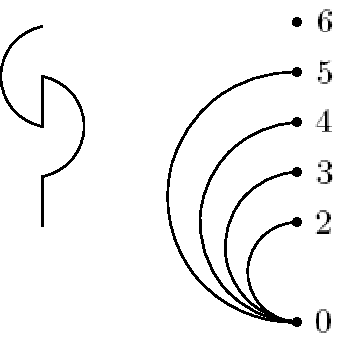
\includegraphics[width=0.2\textwidth]{figures/figure40.pdf}
\caption{\small The Steenrod action on the cohomology of $R$.}
\end{wrapfigure}
The map \begin{tikzcd}[column sep=small]\RP^\infty \rar[stable]& \pt{\RP^\infty}\end{tikzcd} is interesting because it doesn't exist unstably; constructing it involves the same game as the shifting of components we played when constructing the $J$-homomorphism.  The cohomology of $R$ has a class $x_0$ in dimension zero coming from $S^0$ and then a class $x_k$ in dimension $k \ge 2$ coming from $H^* \Suspend \RP^\infty$, and $\Sq^k x_0 = x_k$ for all $k$!  The reason for studying $R$ is that $bo_* R$ is very simple; in fact, $bo \sprod R$ is a bouquet of Eilenberg-Maclane spectra:
\[
bo \sprod R \simeq \bigvee_{k \ge 0} \Suspend^{4k} H\Z_{(2)},
\]
and
\[
bo \langle 4, \infty \rangle \sprod R \simeq \bigvee_{k \ge 1} \Suspend^{4k} H \Z_{(2)} \vee \bigvee_{k \ge 1} \Suspend^{4k+2} H\Z_2
.\]
And so we computed $j \sprod R$ from the sequence
\begin{ctikzcd}
j \sprod R \rar & bo \sprod R & \rar["\Psi^3 - 1"] & bo \langle 4, \infty \rangle \sprod R.
\end{ctikzcd}

It's a rational calculation; there's just not that much to do.  The result is striking: $j \sprod R$ is almost not there at all.
\[
\begin{array}{ccccc}
& j \sprod R & bo \sprod R & & bo \langle 4, \infty \rangle \sprod R \\
0 & \Z_{(2)} & \Z_{(2)} \\
1 \\
2 \\
3 \\
4 & & \Z_{(2)} & \stackrel{=}{\to} & \Z_{(2)} \\
5 & \Z_2 \langle \sigma_1 \rangle \\
6 & & & & \Z_2 \\
7 & \Z_2 \langle \tau_1 \rangle \\
8 & & \Z_{(2)} & \stackrel{\cdot 2}{\to} & \Z_{(2)} \\
9 & \Z_2 \langle \sigma_2 \rangle \\
10 & & & & \Z_2 \\
11 \\
12 & & \Z_{(2)} & \stackrel{=}{\to} & \Z_{(2)} \\
13 & \Z_2 \langle \sigma_3 \rangle \\
14 & & & & \Z_2 \\
15 & \Z_4 \langle \tau_2 \rangle \\
16 & & \Z_{(2)} & \stackrel{\cdot 4}{\to} & \Z_{(2)} \\
17 & \Z_2 \langle \sigma_4 \rangle.
\end{array}
\]
That's it!
\begin{align*}
j_{8k-1}(R) & = \Z_{2^{\nu(k)+1}} \langle \tau_k \rangle & k \ge 1, \\
j_{4k+1}(R) & = \Z_2 \langle \sigma_k \rangle & k \ge 1.
\end{align*}
Now we're really interested in $\RP^\infty$.
\[
\begin{array}{cccc}
& j \sprod \RP^\infty & j \sprod S^0 & j \sprod R \\
0 & \Z & \Z & \Z_{(2)} \\
1 & \Z_2 & \Z_2 \langle \alpha_1 \rangle \\
2 & \Z_2 & \Z_2 \langle \alpha_2 \rangle \\
3 & \Z_8 & \Z_8 \langle j_2 \rangle \\
4 & \Z_2 \langle \sigma_1 \rangle \\
5 & 0 & & \Z_2 \langle \sigma_1 \rangle \\
6 & \Z_2 \langle \tau_1 \rangle \\
7 & \Z_{16} & \Z_{16} \langle j_3 \rangle & \Z_2 \langle \tau_1 \rangle \\
8 & \Z_2 \oplus (\Z_2 \langle \sigma_2 \rangle) & \Z_2 \langle j_4 \rangle \\
9 & \Z_2 \oplus \Z_2 & \Z_2 \oplus \Z_2 & \Z_2 \langle \sigma_2 \rangle \\
10 & \Z_2 & \Z_2 \\
11 & \Z_8 & \Z_8 \langle j_6 \rangle \\
12 & \Z_2 \langle \sigma_3 \rangle & 0 \\
13 & 0 & 0 & \Z_2 \langle \sigma_3 \rangle \\
14 & \Z_2 \langle \tau_2 \rangle  & 0 \\
15 & \Z_{32} & \Z_{32} \langle j_7 \rangle & \Z_4 \langle \tau_2 \rangle \\
16 & \Z_2 \oplus \Z_2 \langle \sigma_4 \rangle & \Z_2 \langle j_8 \rangle.
\end{array}
\]
AND AN UNREADABLE ROW.  Various things could happen, but in fact nothing else does:
\[
j_* \RP^\infty \cong j_* \oplus \langle t_k, \sigma_k \rangle.
\]
So now we've computed the $E^2$-term and the ``abutment'' of the Atiyah-Hirzebruch spectral sequence $H^*(\RP^\infty; j_*) \Rightarrow j_* \RP^\infty$.  A picture is attached of what the filtration looks like; we've really reached the outer limits of human comprehension here.  Note that each of the dots is a $\Z_2$, so a non-zero differential connecting two dots is death to both of them.  So you get to $E^\infty$ from $E^2$ pretty quickly, and you can see a good deal of $E^\infty$ in this picture.

Remember what we had: there were three exact couples
\begin{ctikzcd}
\pi_* \Loops^n S^n \dar\rar & \pi_* \Loops^{n+1} S^{n+1} \dar\rar & \pi_* \Loops^{n+1} S^{2n+1} \dar \\
\pi_*^S \RP^{n-1} \dar\rar & \pi_*^S \RP^n \dar\rar & \pi_*^S S^n \dar\\
j_* \RP^{n-1} \rar & j_* \RP^n \rar & j_* S^n,
\end{ctikzcd}
and the last spectral sequence can be written out completely; it's the chart.  Today we'll talk about two problems: first, given a class $v \in j_* \RP^\infty$, where can be find a representative, which we will denote $H(v)$, in $j_*$? and secondly, how do classes in $j_* \RP^\infty$ pull back to $\pi_*^S \RP^\infty$, or even better, to the EHP sequence?
\begin{ctikzcd}
S^k \ar[ddr,end anchor=north west]\drar[end anchor=north west]\rar & j \sprod \RP^\infty \\
& |[inner xsep=0pt]|j \sprod \RP^3\uar\dar \\ 
& |[inner xsep=0pt]|j \sprod S^3.
\end{ctikzcd}
Recall $j_* \RP^\infty = j_* \oplus \langle \tau_k, \sigma_k$, and $j_*$ contained elements $\alpha_k$ of order $2$ and elements $j_k$.  Recall also that $\alpha_k$ were often not generators; for example, $\alpha_3 = 4j_2$.  So we introduce the notation that $\alpha_{k/i}$ is an element such that $2^{i-1} \alpha_{k/i} = \alpha_k$.  For example, $\alpha_4 = 8 \sigma$, so $\alpha_{4/2} = 4 \sigma$, $\alpha_{4/3} = 2\sigma$, $\alpha_{4/4} = \sigma$, and $\alpha_{4/1} = \alpha_4$.  With this notation we can get all the classes in the image of $J$ except $j_{4k}, j_{4k+1} \in \pi_{8k} J, \pi_{8k+1} J$.  Then the representatives of $j^* \RP^\infty$ in this spectral sequence are found as follows:
\begin{align*}
H(\alpha_{k/i}) & = \alpha_{k-i} \\
H(j_{4k+1i}) & = j_{4k+i-1}, & i = 0, 1 \\
H(\sigma_k) & = \nu = j_2 \in \pi_3(J) \\
H(2^i \tau_k) & = j_{i+1}, & i \le \nu(k).
\end{align*}
Some patterns you will observe when you compare this with the picture:
\begin{enumerate}
\item Elements in the image of $J$ are born as early as possible, so they are concentrated on the left of the table.
\item $\sigma_k$s are born as \emph{late} as possible, so they occur to the \emph{right} on their total degree lines.
\item $\tau_k$s are born as late as possible, subject to the requirement that $2^i \tau_k$ are born as late as possible too.
\end{enumerate}
The next question we posed for ourselves was: how does this picture pull back to the EHP sequence and $\pi_*^S = \pi_* QS^0$?  Mahowald's answer is
\begin{thm}(Mahowald)
The image of $\pi_*^S = \pi_* QS^0 \to \pi_*^S \RP^\infty \to j_* \RP^\infty$ contains $\Jtwee_*$, $\sigma_{2^k}$ for $k \ge 1$, and may contain $2^k \tau_k, k \ge 0$ (coming from Kervaire invariant classes; we know that $\theta_2, \ldots, \theta_5$ do exist with $\theta_{k+2} \in \pi^S_{8 \cdot 2^k-2}$), and \emph{nothing else}!
\end{thm}
What does this tell us about our picture?  For elements in the image of $J$, the EHP spectral sequence looks the same as our chart.  Elements in the image $\pi_* J \to \pi_*^S$ are born on the expected spheres (they can't be born earlier than they are here, and Mahowald constructed such elements in the EHP spectral sequence in the right dimensions in his paper) and their Hopf invariants have the right image in $j_* S^n$ under the map of spectral sequences.  In fact, a great deal of the information from various parts of the course can be discerned in the picture.  For example, Hopf invariant 1 is present: if you project
\begin{ctikzcd}
\pi_*^S S^0 \rar & \pi_*^S \RP^\infty \rar & j_* \RP^\infty \rar & j_*  \RP^\infty_n
\end{ctikzcd}
with $n$ odd, then $\pi_*^S S^0 \to j_* \RP^\infty_n = \Z_2$ is the Hopf invariant.  So you have an element of Hopf invariant 1 if you have a survivor in the bottom row.

The issue of the desuspension of $w_n$ (and so of vector fields on spheres) became a picture of differentials off classes in the bottom row of the Atiyah-Hirzebruch spectral sequence for $\pi_*^S \RP^\infty$; the desuspension of $w_n$ is represented by the end of the differential.

The desuspension of $w_n$s brings us to the Kervaire Invariant classes.  Notice in the picture at the $(7, 7)$ position the differential coming in above from the bottom row: INKSCAPE  What you would hope is that $\theta_3 = \frac{1}{2}$ times the desuspension of $w_15$.  So that's part of the wish list for Kervaire invariant classes:
\begin{itemize}
\item $\theta_k \in \pi^S_{2^{k+1}-2}$
\item born on $S^{2^{k+1} - 1 - |j_k|}$
\item Hopf invariant of $j_k$ (or at least having some image in $j_*$ as $j_k$
\item order 2 (since in $j_* \RP^\infty$, $2^k \tau_{2^k}$ has order 2)
\item $\theta_k$ halves a maximal desuspension of $w_{2^{k+1}-1}$
\item no further division by $2$ is possible, because in $j_* \RP^\infty$ further divisors exist, but these are not in the image of $\pi_*^S$
\item detected on the Adams $2$-line.
\end{itemize}
Other things have been done: you could investigate further how the classes that are in $\pi_*^S$ behave in the EHP sequence; for example, you could try to compute $p(j_k)$.  Mahowald's theorem tells good information about when these are nonzero.  Feder, Gittler, and Lan (cite them) have shown other classes for which $p(j_k) = 0$.  But the Kervaire Invariant classes represent a real missing case here, about which relatively little is known.
% >>>
\fi
\BoxedNote{}
